\documentclass[a4paper,12pt]{report}

\usepackage[utf8x]{inputenc}
\usepackage[T2A]{fontenc}
\usepackage[english, russian]{babel}

% Опционно, требует  apt-get install scalable-cyrfonts.*
% и удаления одной строчки в cyrtimes.sty
% Сточку не удалять!
% \usepackage{cyrtimes}

% Картнки и tikz
\usepackage{graphicx}
\usepackage{tikz}
\usetikzlibrary{snakes,arrows,shapes}


% Увы, поля придётся уменьшить из-за листингов.
\topmargin -1cm
\oddsidemargin -0.5cm
\evensidemargin -0.5cm
\textwidth 17cm
\textheight 24cm

\sloppy



% Оглавление в PDF
\usepackage[
bookmarks=true,
colorlinks=true, linkcolor=black, anchorcolor=black, citecolor=black, menucolor=black,filecolor=black, urlcolor=black,
unicode=true
]{hyperref}

% Для исходного кода в тексте
% \newcommand{\Code}[1]{\texttt{#1}}

% Некоторая русификация.
% \usepackage{misccorr} % Oh shi^W^W, оно не работает с report.
\usepackage{indentfirst}
\renewcommand{\labelitemi}{\normalfont\bfseries{--}}

% На дворе XXI век, но пакет listings всё ещё не пашет с русскими комментариями!

% Пакет listings для простой вставки исходников
% \usepackage{listings}
% Параметры оформления
% \lstset{
% showspaces=false,
% showtabs=false,
% frame=single,
% tabsize=4,
% basicstyle=\ttfamily,
% identifierstyle=\ttfamily,
% commentstyle=\itshape,
% stringstyle=\ttfamily,
% keywordstyle=\ttfamily,
% breaklines=true
% }
% Русский в комментариях.
% \lstset{escapebegin=\begin{cyr},escapeend=\end{cyr}}



% А это взято из файла, сгенерённого doxygen
\usepackage{calc}
\usepackage{array}
\newenvironment{Code}
{\footnotesize}
{\normalsize}
\newcommand{\doxyref}[3]{\textbf{#1} (\textnormal{#2}\,\pageref{#3})}
\newenvironment{DocInclude}
{\footnotesize}
{\normalsize}
\newenvironment{VerbInclude}
{\footnotesize}
{\normalsize}
\newenvironment{Image}
{\begin{figure}[H]}
{\end{figure}}
\newenvironment{ImageNoCaption}{}{}
\newenvironment{CompactList}
{\begin{list}{}{
  \setlength{\leftmargin}{0.5cm}
  \setlength{\itemsep}{0pt}
  \setlength{\parsep}{0pt}
  \setlength{\topsep}{0pt}
  \renewcommand{\makelabel}{\hfill}}}
{\end{list}}
\newenvironment{CompactItemize}
{
  \begin{itemize}
  \setlength{\itemsep}{-3pt}
  \setlength{\parsep}{0pt}
  \setlength{\topsep}{0pt}
  \setlength{\partopsep}{0pt}
}
{\end{itemize}}
\newcommand{\PBS}[1]{\let\temp=\\#1\let\\=\temp}
\newlength{\tmplength}
\newenvironment{TabularC}[1]
{
\setlength{\tmplength}
     {\linewidth/(#1)-\tabcolsep*2-\arrayrulewidth*(#1+1)/(#1)}
      \par\begin{tabular*}{\linewidth}
             {*{#1}{|>{\PBS\raggedright\hspace{0pt}}p{\the\tmplength}}|}
}
{\end{tabular*}\par}
\newcommand{\entrylabel}[1]{
   {\parbox[b]{\labelwidth-4pt}{\makebox[0pt][l]{\textbf{#1}}\vspace{1.5\baselineskip}}}}
\newenvironment{Desc}
{\begin{list}{}
  {
    \settowidth{\labelwidth}{40pt}
    \setlength{\leftmargin}{\labelwidth}
    \setlength{\parsep}{0pt}
    \setlength{\itemsep}{-4pt}
    \renewcommand{\makelabel}{\entrylabel}
  }
}
{\end{list}}
\newenvironment{Indent}
  {\begin{list}{}{\setlength{\leftmargin}{0.5cm}}
      \item[]\ignorespaces}
  {\unskip\end{list}}


\title{Расчетно-Пояснительная Записка \\
    \large к курсовой работе на тему: \\ Серверная часть MTA SMTP}
\author{Сычев С.А. ИУ7-32М}

\begin{document}

\maketitle

\tableofcontents

\newpage
\chapter*{Введение}
\addcontentsline{toc}{chapter}{Введение}

Данная работа посвящена разработке серверной части почтового сервера MTA (англ. Message Transfer Agent), использующего протокол SMTP (англ. Simple Mail Transfer Protocol) - сетевой протокол, предназначенный для передачи электронной почты в сетях TCP/IP. 

Цель работы: спроектировать, разработать и протестировать серверную часть почтового SMTP-сервера (MTA), обеспечивающую локальную доставку сообщений и их добавление в очередь удаленной доставки. 

Дополнительные условия:
\begin{itemize}
\item Использовать системный вызов \texttt{poll()};
\item Использовать рабочие процессы;
\item Журналирование осуществлять в отдельном процессе.
\item Требуется проверять обратную зону DNS.
\end{itemize}

Основные задачи:
\begin{enumerate}
    \item Анализ ...;
    \item Проектирование ...;
    \item Реализация SMTP-сервера; 
    \item Тестирование и отладка реализованного программного обеспечения;
    \item Оформление расчетно-пояснительной записки по результатам работы.
\end{enumerate}

\newpage
\chapter{Аналитический раздел}

\section{Протокол SMTP}
SMTP ~-- это сетевой протокол, предназначенный для передачи писем электронной почты в сетях TCP/IP. SMTP впервые был описан в RFC 821 (1982 год), а последнее обновление описано в RFC 5321 (2008 год) и включает масштабируемое расширение протокола — ESMTP (Extended SMTP). В настоящее время под протоколом SMTP подразумеваются и его расширения. Протокол SMTP предназначен для передачи исходящей почты с использованием порта TCP 25.

Взаимодействие в рамках SMTP строится по принципу двусторонней связи, устанавливаемой   между отправителем и получателем почтового сообщения. При этом отправитель инициирует соединение и посылает запросы, а получатель - отвечает на эти запросы. Таким образом, отправитель выступает в роли клиента, а получатель - сервера.

\subsection{Команды протокола SMTP}

Команды протокола SMTP начинаются с названий - ключевых слов, указывающих, какую операцию хочет осуществить клиент.
За ключевым словом следуют, отделенные пробелом, параметры. Конец команды обозначается последовательностью символов \textbackslash r\textbackslash n - обозначаемой CRLF. 

Ниже представлен список базовых SMTP-команд:
\begin{itemize}
	\item \textbf{HELO [доменное имя клиента] CRLF} - Открывает SMTP сессию. В RFC 2821 рекомендуется использовать команду HELO, только если программное обеспечение не поддерживает команду EHLO.
	\item \textbf{EHLO [доменное имя клиента] CRLF} - Открывает ESMTP сессию. В ответ на эту команду сервер сообщает, готов ли он к продолжению диалога.
	\item \textbf{MAIL FROM: <адрес\_отправителя> CRLF} - Сообщает адрес отправителя письма. Команда MAIL должна быть выполнена для письма только один раз и только после успешного выполнения команды EHLO или HELO.
	\item \textbf{RCPT TO: <адрес\_получателя> CRLF} - Сообщает адрес получателя письма. Доставка сообщения возможна, только если указан хотя бы один адрес получателя. Команда RCPT может быть выполнена только после успешного выполнения команды MAIL и должна быть повторена для каждого получателя письма.
	\item \textbf{DATA CRLF} - Сообщает о готовности ввода текста письма. Команда DATA может быть выполнена только после успешного выполнения хотя бы одной команды RCPT. После успешного ответа сервера, клиент начинает передачу текста письма, с учетом заголовков. Сервер определяет окончание текста письма по последовательности: CRLF . CRLF
	\item \textbf{RSET CRLF} - Сброс SMTP соединения. Команда RSET аннулирует все переданные до нее на сервер данные.
	\item \textbf{VRFY <адрес> CRLF} - Проверяет наличия указанного в качестве аргумента почтового адреса.
	\item \textbf{QUIT CRLF} - Закрывает SMTP сессию.
\end{itemize}

Существуют также и другие команды ESMTP, однако в данной работе они не рассматриваются. 

\subsection{Ответы SMTP сервера}

Ответ SMTP сервера состоит из кода ответа, за которым через пробел следует дополнительный текст. Код служит индикатором состояния сервера и делится на четыре группы:
\begin{itemize}
	\item \textbf{2xx} - команда выполнена успешно;
	\item \textbf{3xx} - ромежуточный положительный результат. Команда принята, но сервер ожидает от клиента дополнительные данные для завершения операции;
	\item \textbf{4xx} - исполнение команды временно невозможно. Команда не может быть выполнена, но проблема может быть устранена;
	\item \textbf{5xx} - исполнение команды невозможно.
\end{itemize}

Если ответ сервера состоит из нескольких строк, то каждая из них начинается кодом, который отделяется от сопровождающего текста не пробелом, а символом "минус"\ (-). В последней строке номер отделяется от текста пробелом. Каждая строка ответа, как и строки команд, заканчивается последовательностью CRLF.

\section{Преимущества и недостатки использования системного вызова poll.}
TODO

Системный вызов poll, по сравнению с другими системными вызовами опроса сокетов имеет следующие достоинства: 
\begin{itemize}
	\item Нет активного ожидания на процессоре.
	\item Позволяет обрабатывать больше 1024 клиентов по сравнению с системным вызовом \texttt{select()}.
	\item Не модифицируется структура pollfd, что даёт возможность её переиспользования между вызовами poll() — нужно лишь обнулить поле revents.
	\item Наблюдаемые события лучше структурированы. Например, можно определить отключение удалённого клиента без необходимости чтения данных из сокета.
\end{itemize}

К его недостаткам можно отнести:
\begin{itemize}
 	\item Poll отсутствует на некоторых платформах (в основном старых). 
	\item Невозможнось определить, какие именно дескрипторы сгенерировали события, без полного прохода по всем наблюдаемым структурам и проверки поля revents. (Проблема так-же в том, что в ядре данная операция реализована так-же). 
	\item Как и при использовании select, нет возможности динамически менять наблюдаемый набор событий. 
\end{itemize}

TODO ВСТАВИТЬ ССЫЛКУ ["select/poll/epoll: практическая разница"]

\section{Преимущества и недостатки использования многопроцессного подхода обработки подключений.}
TODO

\begin{itemize}
 	\item ...
	\item ...
\end{itemize}

К минусам использования этого подхода относятся:
\begin{itemize}
    \item ...
    \item ...
\end{itemize}


\section{Сущности предметной области}

TODO

\newpage
\chapter{Конструкторский раздел}

\section{Конечный автомат состояний сервера}

На рис.~\ref{fig:fsm} изображен конечный автомат разрабатываемой серверной части SMTP сервера. 

\begin{figure}[H]
	\centering
	\includegraphics[width=\textwidth]{build/fsm.pdf}
	\caption{Конечный автомат состояний сервера}
	\label{fig:fsm}
\end{figure}

\section{Синтаксис команд протокола}

\section{Описание основных структур данных}

\section{Обработка соединений в одном потоке выполнения}

\section{Связь основной программы и процесса журналирования}

\section{Хранение почты}

\chapter{Технологический раздел}

\section{Язык программирования и библиотеки}

Для написания исходного кода SMTP сервера использовался язык C стандарта C99.

Помимо стандартных библиотек были использованы:
\begin{itemize}
    \item TODO - все из sys 
    \item libconfig - библиотека для чтения файлов конфигурации.  
    \item Autogen - библиотека для автоматической генерации конечного автомата состояний.
    \item PCRE - библиотека для работы с регулярными выражениями. 
    \item CUnit - библиотека для модульного тестирования.
\end{itemize}


\section{Платформы и компиляторы}

Для сборки использовался компилятор gcc, со следующими флагами: 
\begin{lstlisting}
-std=c99 -g -g3 -O0 -Wall -Werror -pedantic -D\_GNU\_SOURCE
\end{lstlisting}
Программное обеспечение разрабатывалось, собиралось и тестировалось на виртуальной машине с ОС Ubuntu 16.04, с двухядерным процессором и 4 ГБ оперативной памяти. 


\section{Сборка}
Сборка осуществляется при помощи утилиты Make. Применен иерархический подход. Сценарии сборки описаны в трех Makefile-ах. 
\begin{enumerate}
	\item Makefile для сборки и тестирования сервера - расположен в каталоге \textbf{/server/src} и отвечает за непосредственную сборку и тестирование сервера. 
	\item Makefile для сборки отчета - расположен в каталоге \textbf{/server/report} и отвечает за сборку данного отчета. 
	\item Корневой Makefile - расположен в каталоге \textbf{/server}, объединяет функции двух предыдущих, имеет общие цели для сборки сервера, его тестирования и генерации отчета, по итогам тестирования. 	
\end{enumerate}

\section{Визуализация сценариев сборки}
В данном разделе приведена визуализиция Makefile-ов, используемых для сборки и тестирования сервера и отчета. 
Визуализация корневого Makefile-а не приводится так как она во многом повторяет указанные ранее. 
\begin{figure}[H]
	\centering
	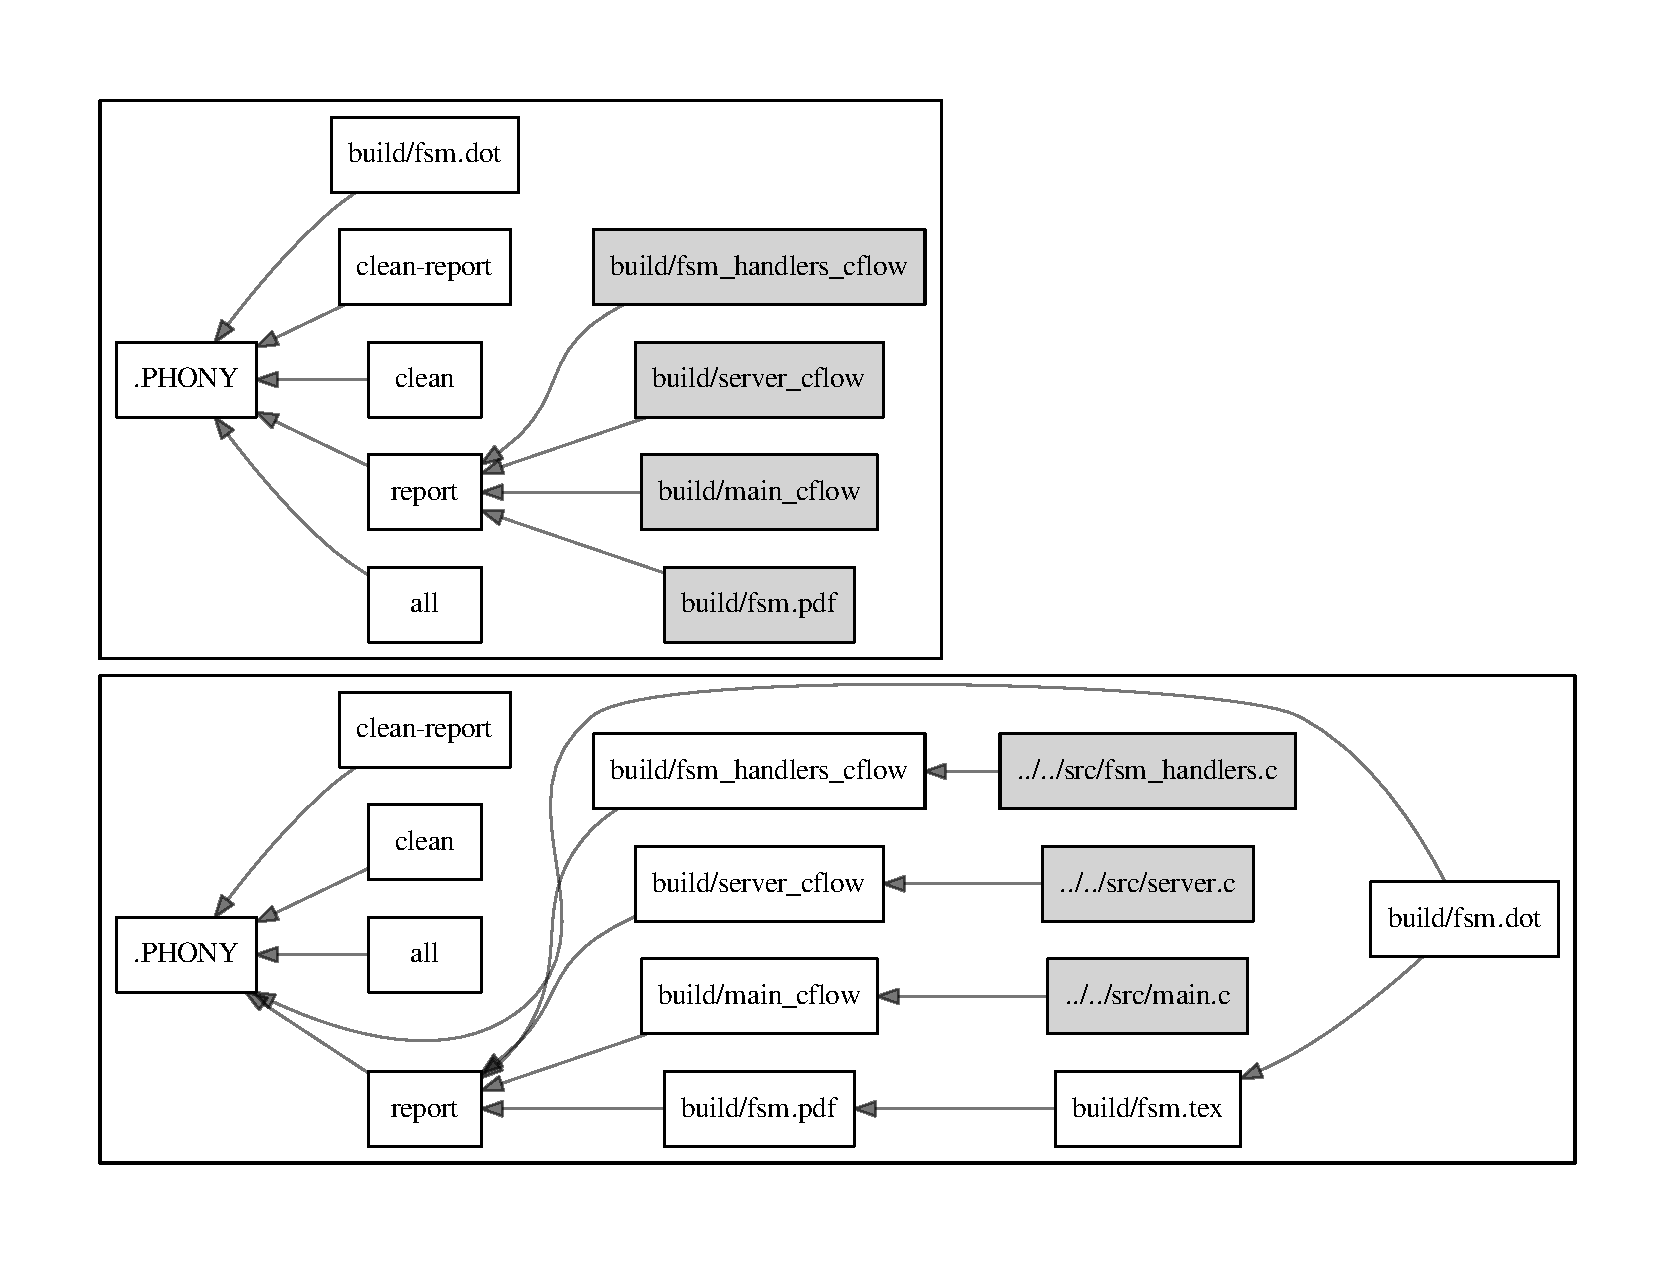
\includegraphics[width=\textwidth]{make_pdfs/report_make.pdf}
	\caption{Визуализация сценария сборки отчета}
	\label{fig:make2}
\end{figure}

\begin{figure}[H]
	\centering
	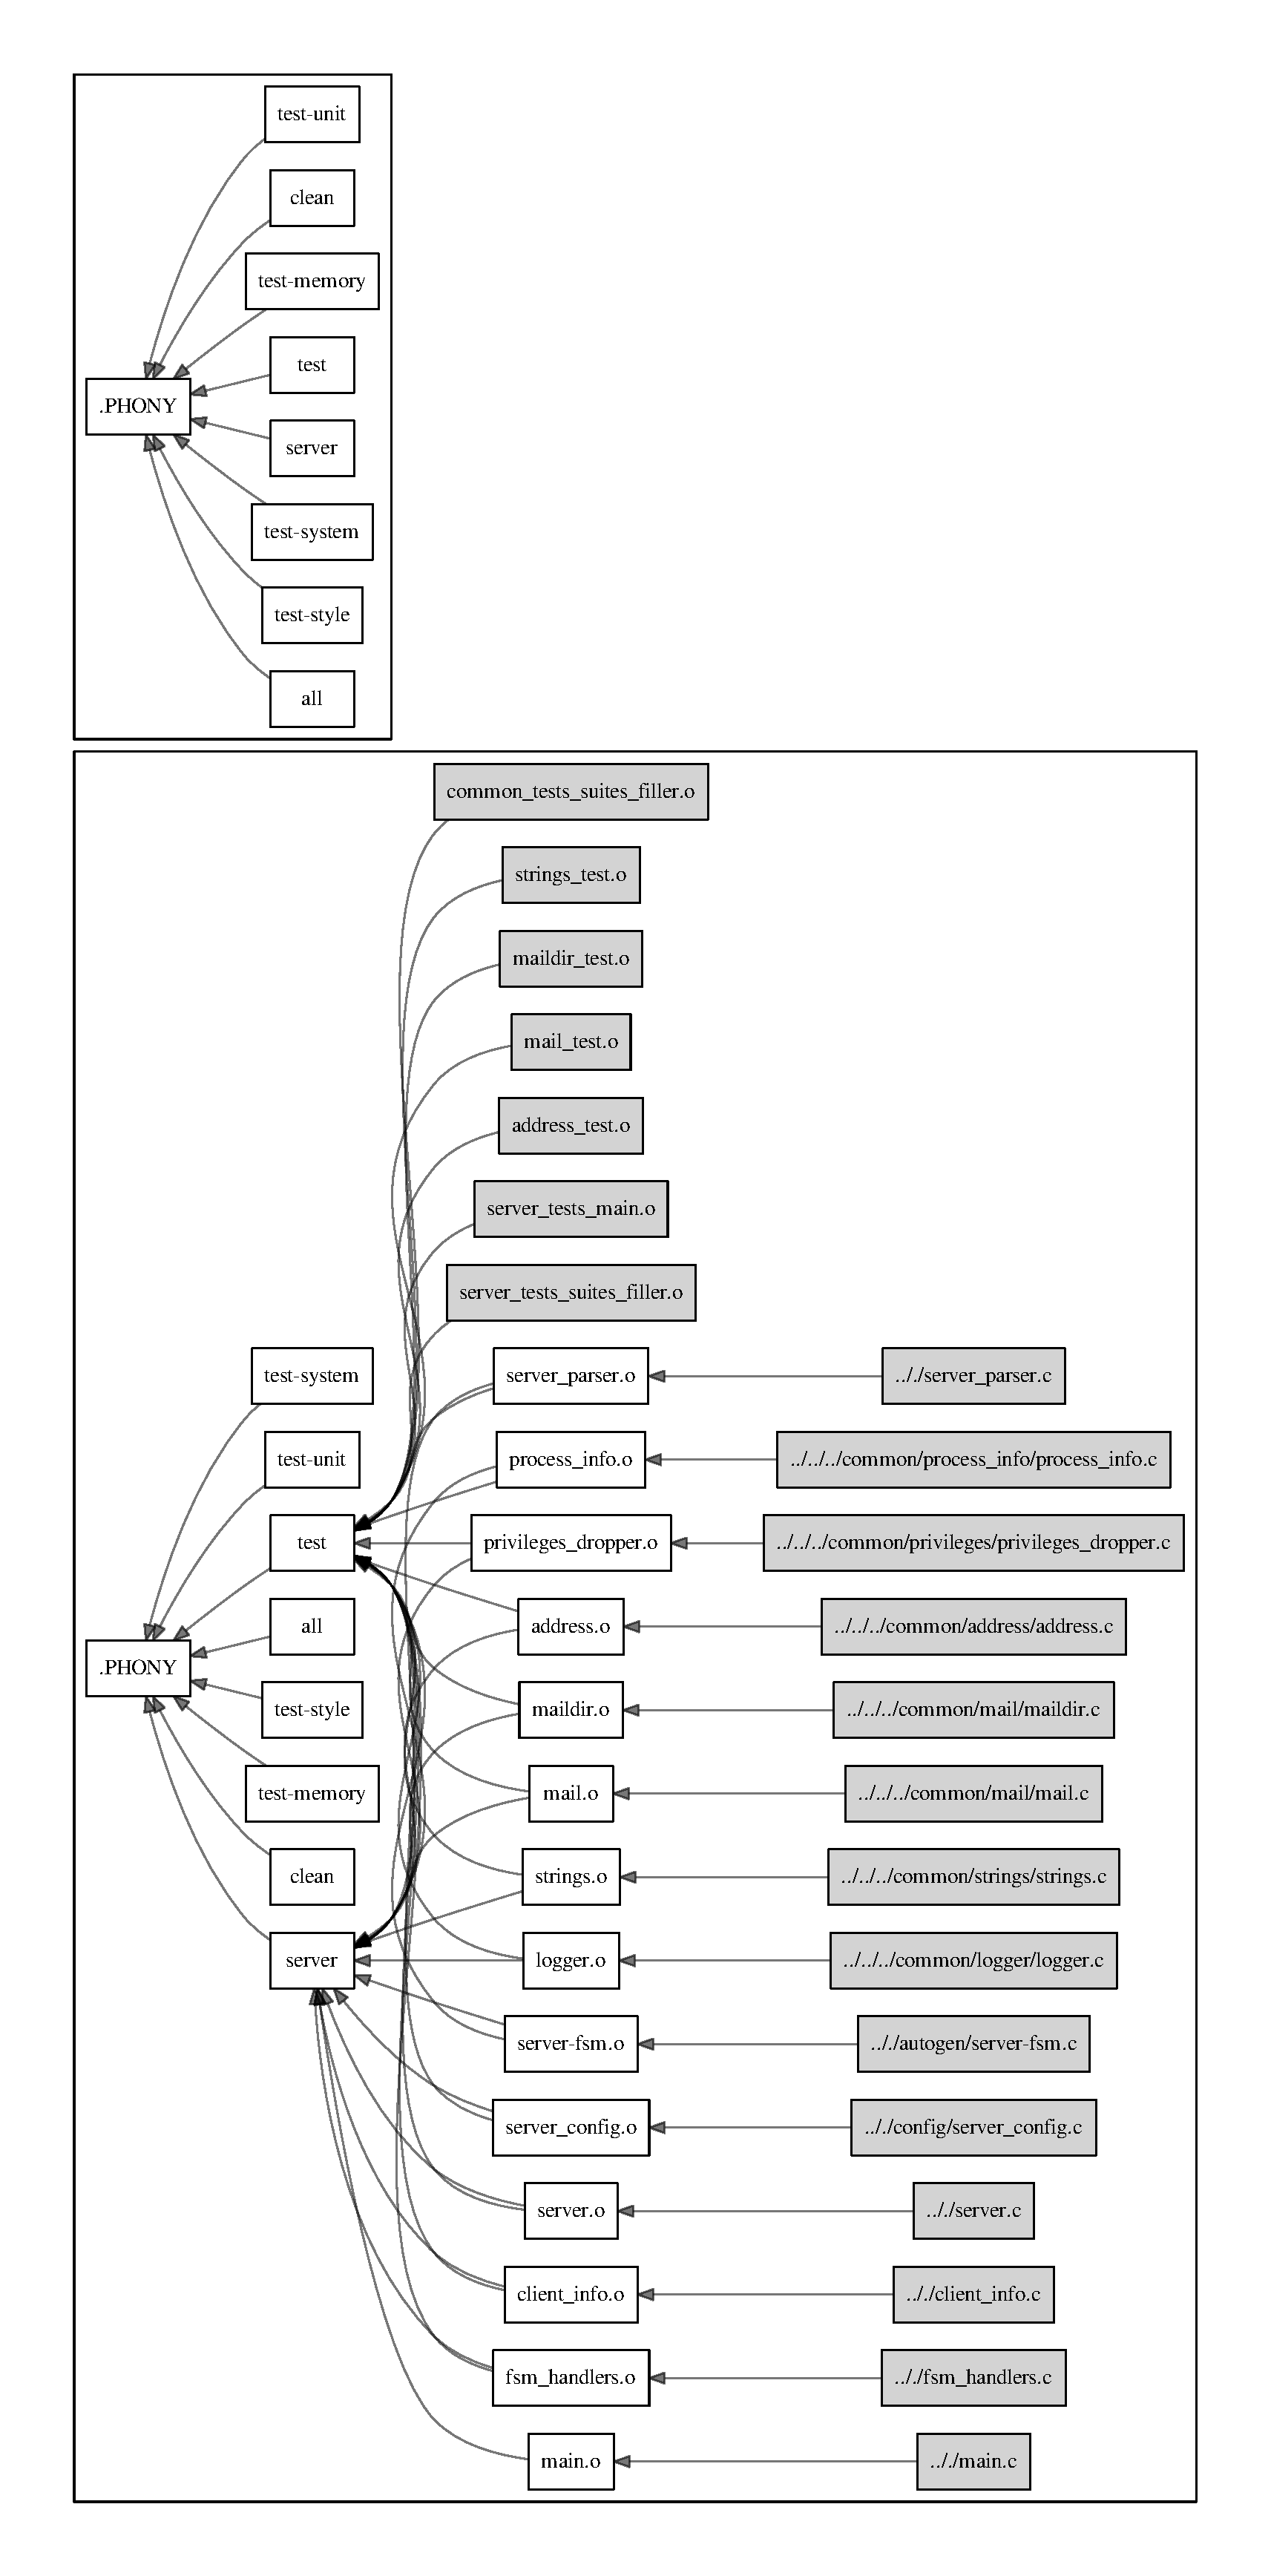
\includegraphics[width=0.7\textwidth]{make_pdfs/server_make.pdf}
	\caption{Визуализация сценария сборки и тестирования сервера}
	\label{fig:make1}
\end{figure}

\section{Кодогенерация}
Для ускорения разработки конечного автомата сервера была применена библиотека autogen. 

Из .def файла с описанием конечного автомата был сгенерирован код, осуществляющий все переключения между состояниями. 

Далее потребовалось лишь написать обработчики переходов. 

Файл, на основании которого был сгенерирован автомат приведен на листинге ниже:
\lstinputlisting[basicstyle=\tiny]{../../src/autogen/server.def}

\section{Документация}
TODO Docsygen

\section{Конфигурация}
Для конфигурирования сервера, используется конфигурационный файл, путь до которого необходимо передавать как параметр командной строки при запуске сервера. 

Для чтения файла конфигурации используется библиотека: \textbf{libconfig}.

В файле конфигурации задаются: 
\begin{itemize}
	\item version - версия файла конфигурации, необходима, чтобы отличить новые версии конфига, в случае дальнейшей работы над проектом.  
	\item port - порт, на котором будет слушать сервер.  
	\item local\_domain - почтовый домен, который сервер будет считать локальным (и письма будут записываться в соответствии с maildir).
	\item log\_filename - имя файла с логом. 
	\item maildir - базовая директория для записи писем.
	\item max\_process\_cnt - максимальное количество рабочих процессов (без учета логгера). 
\end{itemize}


Ниже привезен пример файла конфигурации:
\lstinputlisting{../../src/server.ini}

\section{Графы вызова функций}
Ниже приведены графы вызова функций для точки входа (\textit{main.c}), основного серверного кода (\textit{server.c}) и обработчиков переходов состояний (\textit{fsm\_handlers.c}). Из графов для большей наглядности удалены обращения к следующим функциям: 

\lstinputlisting{cflowignore.txt}

\begin{figure}[H]
	\includegraphics[width=0.7\textwidth]{build/main_cflow0.pdf}
	\caption{Граф вызовов. Точка входа}
	\label{fig:cflow1}
\end{figure}

\begin{figure}[H]
	\includegraphics[width=1\textwidth]{build/server_cflow0.pdf}
	\caption{Граф вызовов. Основной код сервера}
	\label{fig:cflow2}
\end{figure}
\begin{figure}[H]
	\includegraphics[width=1\textwidth]{build/fsm_handlers_cflow0.pdf}
	\caption{Граф вызовов. Обработчики переходов состояний}
	\label{fig:cflow3}
\end{figure}

\newpage
\section{Модульное тестирование}
Для модульного тестирования функций сервера в работе используется библиотека CUnit.

Модульными тестами покрыто подавляющее большинство функций из библиотек, размещенных в common, т.к. они широко используются в коде серверной части.

Результаты тестирования привидены на листинге ниже: 
\lstinputlisting{../../src/test-unit.out}

\section{Системное тестирование}
Системное тестирование реализовано в виде скрипта на языке Python. Использован SMTP клиент из стандартной библиотеки Python. 

Все тесты устроены следующим образом: 
\begin{itemize}
	\item Подготавливаются данные для отправки письма/писем. 
	\item SMTP клиент подключается к серверу и выполняет отправку одного или нескольких писем. 
	\item Производится проверка корректности записи писем (вплоть до посимвольной проверки содержимого файла).
\end{itemize}

При этом до запуска тестов, автоматически запускается сервер, а после завершения - отправляется сигнал SIGINT, для корректного завершения работы. 

Реализованы следующие системные тесты: 
\begin{itemize}
	\item Простой тест с отправкой небольшого письма одному получателю.  
	\item Тест с отправкой письма, размером ~1МБ.  
	\item Тест с отправкой письма с несколькими получателями, в т.ч. с локальным/удаленным почтовым доменом.
	\item Тест с отправкой нескольких писем в рамках одной SMTP сессии. 
\end{itemize}

Результаты системного тестирования приведены ниже:
\lstinputlisting{../../src/test-system.out}

\section{Тестирование утечек памяти}
Для тестирования утечек памяти использовалась утилита valgrind.

При выполнении основного сценария сборки и тестирования проводится автоматический запуск модульных и системных тестов под valgrind. 

Результаты проверки модульных тестов приведены на листинге ниже, утечек памяти не обнаружено: 
\lstinputlisting{../../src/test-memory.out}


Результаты проверки системных тестов приведены на листинге ниже, утечек памяти не обнаружено: 
\lstinputlisting{../../src/test-system-memory.out}


\section{Тестирование стиля кодирования}

В качестве стиля кодирования был выбран Google С++ style [https://google.github.io/styleguide/cppguide.html] с несколькими незначительными изменениями. 
 
Для проверки стиля кодирования использовалась утилита от Google с открытым исходным кодом: cpplint.py [https://github.com/google/styleguide/tree/gh-pages/cpplint]. 

В утилиту были внесены незначительные изменения (для отмены нескольких правил, которые были сочтены излишними). Также применялся флаг для установки максимальной длины строки в 120 символов, вместо стандартных 80.

В ходе автоматической проверки стилевых ошибок не обнаружено, результаты проверки приведены на листинге ниже: 
\lstinputlisting{../../src/test-style.out}

\clearpage
\chapter*{Заключение}
\addcontentsline{toc}{chapter}{Заключение}

TODO

\newpage
\chapter*{Список литературы}
\addcontentsline{toc}{chapter}{Список литературы}

\begin{enumerate}
	\item Статья "select/poll/epoll: практическая разница" [Электронный ресурс] Режим досутпа: URL: https://habr.com/ru/company/infopulse/blog/415259/
	
\end{enumerate}

1) http://www.faqs.org/rfcs/rfc5321.html - RFC 5321 (Спецификация протокола SMTP)
2) http://cunit.sourceforge.net/documentation.html - документация cunit 
3) https://github.com/google/styleguide/tree/gh-pages/cpplint - github cpplint
4) https://habr.com/ru/post/148948/ - libconfig "Конфигурационные файлы. Библиотека libconfig"
5) https://www.pcre.org/ - офф сайт pcre 
6) 

\lstlistoflistings

\end{document}




